To afford accurate crowd animations for player visualization, a humanoid character model with animations is employed. The complete set includes idle and walking animations. The crowd members are generated and distributed at random locations in the layout based on the configurations set by the player. Destinations and distributions for locations of crowd members can be modified and constrained by the architect or designer as well. To ensure accurate navigation, the navigation mesh of the environment and path plans for each member are recomputed after every level change and before a simulation is started.

We used an agent-based model for simulating crowd steering. We have also tried to incorporate different steering decision behaviours observed in the crowd at the time of emergencies. For instance during a fire, people tend to follow each other in order to find the exits or people tend to follow the exit signs more stringently than in their day to day lives. While going to their destination, if an member sees an exit which is closer than their assigned one their navigation goal switches to the closer observed goal. The members also change their destination and path when a big group of other members are moving towards a certain destination. So in a sense, the members follow the crowd unless they themselves see an exit.

To afford rigorous and complete testing across dynamics and behaviours, the crowds are parametrized for aggression, homogeneity, and density.  These parametrizations and a formal definition of a crowd are provided in the rest of this section.

\begin{itemize}

\item \textbf{Level of Aggression (LoA)} - Three degrees of aggression are provided; low, medium and high. The aggression degree determines the speed and acceleration of different members in the crowd. As the aggression level increases, the distribution of aggressive people in the crowd also increases. Fixed probabilities are associated with the low, medium, and high degrees and are used to assign appropriate speeds to the members. The mapping of degrees of aggression to speeds and accelerations can be seen in Table~\ref{table:aggression-levels-speeds} and Table~\ref{table:aggression-levels-accels} respectively.

\item \textbf{Level of Homogeneity (LoH)} - Three classes of homogeneity are available to the player: low, medium, and high. Changing this configuration changes the distribution of the radii of the crowd members.  Low means that there is a low probability in the variety of members that have a radius other than the average one. This helps the player to identify how well their design handles different body shapes in a crowd.

\item \textbf{Level of Service (LoS)} - There are six Levels of Service available to the player. Level of Service is used by traffic engineers to measure the quality of traffic flow both for automotive and pedestrian applications. LoS classes are typically given a grade level (from A-F), which are summarized in Table~\ref{table:los}. 

\end{itemize}

Examples of these parametrizations can be seen in Figure~\ref{fig:crowd-parameter-ex}.

\begin{figure*} 
	\begin{tabular}{c c c} 
	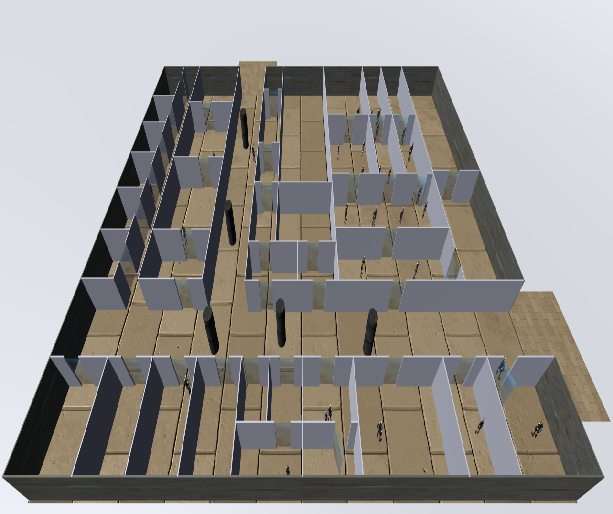
\includegraphics[width=0.31\textwidth]{images/LoS_A_lowest_density.png} & 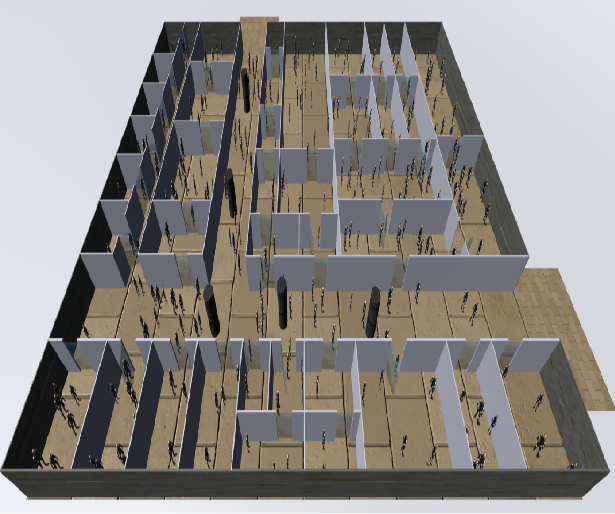
\includegraphics[width=0.31\textwidth]{images/LoS_F_highest_crowd_density.png} & 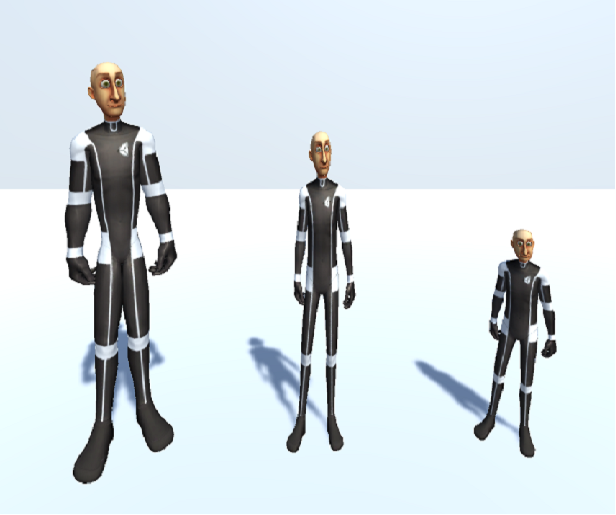
\includegraphics[width=0.31\textwidth]{images/LevelOfHomogeneity.png} \\
	(a) & (b) & (c)
	\end{tabular}
	\caption{\label{fig:crowd-parameter-ex}Crowd configuration and simulation: a) High Level of service, b)Low level of service, c)Level of Homogeneity}
\end{figure*}

\begin{table}
	\centering
	\begin{tabular}{||c c ||}
		\hline
		LOS & Crowd Density (people/square unit)\\ [0.5ex] 
		\hline\hline
		A & $<$=0.27  \\ 
		\hline
		B & 0.31 - 0.43 \\
		\hline
		C & 0.44 - 0.72  \\
		\hline
		D & 0.72 - 1.08 \\
		\hline
		E & 1.09 - 2.17 \\
		\hline
		F & $>$ 2.17 \\ 
		\hline
	\end{tabular}
	\caption{LoS classifications and their associated densities.}
	\label{table:los}
\end{table}

We formally denote a crowd $C = \langle g, k, l \rangle$ that describes the crowd related parameters where g, k, l denote LoS, LoA, LoH respectively.
A gamified environment area is formally described as multiple heterogeneous sub areas. Let $y_{j}$ be a random variable for sub area j with a value in range [$g_{min},g_{max}$]. Let, $n_{j}$ be the number of members in the sub area j.

\begin{equation}
\mathbf{n_{j}} = Q_{j} \times \delta \times x_{i} 
\end{equation}

where, $Q_{j}$ is the area of sub area j and $\delta$ is the normalization constant.
We described a transformation/mapping function that converts the crowd configuration to an instance of member $A = \{ a \}$ where each member $a = \langle \mathbf{p}, \mathbf{v},\mathbf{f}, \mathbf{r},\mathbf{h},\mathbf{m} \rangle$ where p = position vector ($\hat{x_{a}},\hat{y_{a}},\hat{z_{a}}$), v = speed, r = radius, h = height, f = acceleration. $\hat{x_{a}}$ and $\hat{z_{a}}$ are random variables in range [$x_{min_{j}}$,$x_{max_{j}}$] and [$z_{min_{j}}$,$z_{max_{j}}$] respectively where $x_{min_{j}}$,$x_{max_{j}}$,$z_{min_{j}}$,$z_{max_{j}}$ are the four extreme coordinates of sub square area j.

\begin{table}
\centering
	\begin{tabular}{||c c c ||} 
	\hline
	k & $x_{i}$ & $v_{a}$\\ [0.5ex] 
	\hline\hline
	Low & $<$=0.7 & $S+ SLOW\times x_{i}$ \\ 
	\hline
	Low & $>$0.7 & $S+ SHIGH\times x_{i}$\\
	\hline
	Medium & $<$=0.5 & $S+ SLOW\times x_{i}$ \\
	\hline
	Medium & $>$0.5 & $S+ SHIGH\times x_{i}$\\
	\hline
	High & $<$=0.7 & $S+ SHIGH\times x_{i} $\\
	\hline
	High & $>$ 0.7 & $S+ SLOW\times x_{i}$\\
	\hline
	\end{tabular}
	\caption{\label{table:aggression-levels-speeds} Speed mapping for aggression levels. Let, $x_{i}$ be the random variable for member i whose value is in the range [0,1]. SLOW and SHIGH are higher and lower aggression factors for speed respectively. S is the speed constant.}
\end{table}

\begin{table}
\centering
	\begin{tabular}{||c c c ||} 
	\hline
	k & $x_{i}$ & $f_{a}$\\ [0.5ex] 
	\hline\hline
	Low & $<$=0.7 & $F+ ALOW\times x_{i}$ \\ 
	\hline
	Low & $>$0.7 & $ F+ AHIGH\times x_{i} $\\
	\hline
	Medium & $<$=0.5 & $F+ ALOW\times x_{i}$ \\
	\hline
	Medium & $>$0.5 & $F+ AHIGH\times x_{i}$\\
	\hline
	High & $<$=0.7 & $F+ AHIGH\times x_{i} $\\
	\hline
	High & $>$ 0.7 & $F+ ALOW\times x_{i}$\\
	\hline
	\end{tabular}
	\caption{\label{table:aggression-levels-accels} Acceleration mapping for aggression levels. ALOW and AHIGH are higher and lower aggression factor for acceleration respectively. F is the acceleration constant.}
\end{table}

Formally, Level of Homogeneity is defined in terms of M,H,R as each crowd member's mass, height, and radius respectively. 
Let $ \alpha , \beta, \gamma $ be heterogeneity factor for mass, height and radius respectively.  The mapping of level to these factors can be found in Table~\ref{table:homogeneity-levels}.

\begin{table}
\centering
	\begin{tabular}{||c c c c c||} 
	\hline
	l & $x_{i}$ & $m_{a}$ & $h_{a}$ & $r_{a}$\\ [0.5ex] 
	\hline\hline
	Low & $<$=0.7 & $M\times \alpha \times x_{i} $ & $h\times \beta \times x_{i}$ & $r\times \gamma \times x_{i} $ \\ 
	\hline
	Medium & $<$=0.5 & $ M\times \alpha \times x_{i}$ & $h\times \beta \times x_{i}$ & $r\times \gamma \times x_{i}$\\
	\hline
	High & $<$=0.3 & $M\times \alpha \times x_{i}$ & $h\times \beta \times x_{i} $ & $r\times \gamma \times x_{i} $\\
	\hline
	\end{tabular}
	\caption{\label{table:homogeneity-levels} Height, radius, and mass mapping for aggression levels.}
\end{table}